\subsection{Data Normalization}
\label{sec:DataNormalization}
When comparing multiple entries in a dataset, it might be beneficial to normalize such to obtain a basis for equal comparison.
In the case of numbers being written and detected, such as ours, there might be differences in the colors of the characters when different pens/pencils are used.
This can create unwanted differences between elements in a category, which are else identically, and hence lead to false predictions.
Two normalization algorithms where hence implemented.
These are, min-max normalization and z-score standardization.

Figure \ref{fig:normalization_test_pre-post} shows the result when cross validation is carried out on the data from the 16 people in the class.
In figure \ref{fig:normalization_test_pre-post}, each individual is tested up against the rest of the group without contributing to the training set themselves. 
The two types of normalization are performed both before and after the data reduction using PCA.


\begin{figure}[H]
\centering
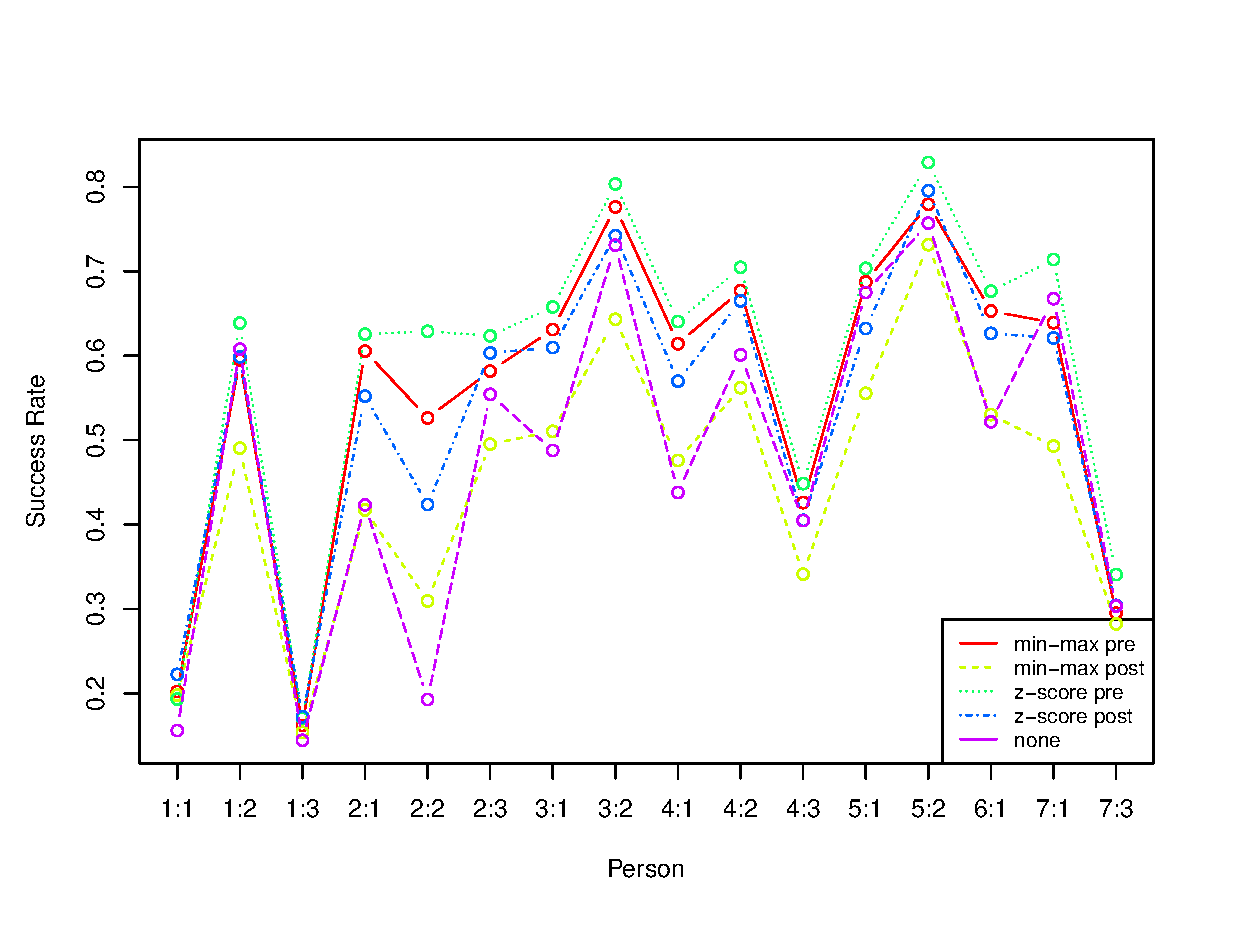
\includegraphics[width = 0.95 \textwidth]{graphics/graph_normalization_allppl}
\caption{Success rate for detection of characters of on person when not in the training set. 
Data normalized before (pre) and after (post) dataset reduction using PCA.
PCA was set to ensure that 80\% of all variance was included in the data set and K as 19.
The person tested for is given as 'Group':'Member'.
It was tested with 16 people.}
\label{fig:normalization_test_pre-post}
\end{figure}

The mean success rate of figure \ref{fig:normalization_test_pre-post} is listed in table \ref{tab:meanSuccess_normalization_test_pre-post}.
From both the graph and table, it can be concluded that the z-score standardization before the PCA reduction performs, on average, at least 3\% better than the other methods.

The figure \ref{fig:normalization_test_pre-post} also shows that in general all three normalizations, except for the min-max normalization after PCA reduction, is on average, yielding a higher number of correct predictions.

The normalization before the PCA reductions yields a better result in all cases. 
This may be because it enables the PCA to find the features being more responsible for the decision of which category a element belongs to. 
Some of the performance improvement can be because of features of a low variance in their measured value, have a larger relevance as to what the actual category of the elements are.


\begin{table}[H]
\centering
\begin{tabular}{|l|r|}\hline
% 0.5532031 0.4493750 0.5874687 0.5339844 0.4791094
Normalization Method & Mean Success \\ \hline
Min-Max Normalization Pre & 55.3 \% \\ \hline
Min-Max Normalization Post & 44.9 \% \\ \hline
Z-Score Normalization Pre & 58.7 \% \\ \hline
Z-Score Normalization Post & 53.4  \% \\ \hline
No Normalization & 47.9 \% \\ \hline
\end{tabular}
\caption{Mean success rates for normalization test as seen in figure \ref{fig:normalization_test_pre-post}.}
\label{tab:meanSuccess_normalization_test_pre-post}
\end{table}



\subsubsection{Performance Effect when adding a Filter}



\textbf{Graphs for selection of optimum filter}

The filter size and sigma is from figure \textbf{ref!!} found to be \textbf{hohaha}.
This was then used to generate figure \textbf{ref!!}.

\textbf{Graph with effect of adding filter to the normalized data}



